\documentclass[12pt]{article}
\usepackage[utf8]{inputenc}
\usepackage{amsmath}
\usepackage{amssymb}
\usepackage{fullpage}
\usepackage{hyperref}
\usepackage{siunitx}
\usepackage[overload]{empheq}
\usepackage{float}
\usepackage{graphicx}
\usepackage{indentfirst}
\usepackage{listings}


%==== templates ====
\iffalse
%inserting code
\lstinputlisting[language=Python]{test.m}

%insertng image
\begin{figure}[H]
\centering
\includegraphics[width=0.5\textwidth]{plot}
\caption{Blah}
\label{blahblah}
\end{figure}

%interting table
\begin{table}[H]
\centering
\begin{tabular}{|c c c c|} 
 \hline
 Col1 & Col2 & Col2 & Col3 \\ 
 \hline
 1 & 6 & 87837 & 787 \\ 
 2 & 7 & 78 & 5415 \\
 3 & 545 & 778 & 7507 \\
 4 & 545 & 18744 & 7560 \\
 5 & 88 & 788 & 6344 \\
 \hline
 \end{tabular}
\end{table}
\fi

%==== document specific commands ====

\renewcommand{\vec}[1]{\mathbf{#1}}
\DeclareRobustCommand{\qed}{\blacksquare}


\title{Using Monte Carlo Renormalization Group to study the Ising model on a two dimensional square lattice}
\author{Jixun Ding (SUID: 3624401)}
\date{March 11, 2019}

\begin{document}

\maketitle
\section{Abstract}
Monte Carlo Renormalization Group (MCRG) is a computational method for investigating critical phenomena in thermodynamical systems by combining standard Monte Carlo simulations with real space renormalization
group analysis. In this work, I follow a description of MCRG by Swendsen~\cite{SwendsenDetail} and Binder~\cite{Binder2014}. I apply MCRG to extract critical exponents of the Ising Model on a two dimensional square lattice. Exact critical exponents for the Ising Model in two dimensions are known~\cite{Onsager1944} to be $y_T = 1, y_H = 15/8$. I find that the MCRG method produces results consistent with these known exact values and Swendsen's results. The effect of lattice size, number of coupling constants considered, and number of renormalization group iterations on the accuracy of the MCRG method are discussed.
\section{Introduction}
\subsection{Renormalization Group Formalism}
Consider a Hamiltonian of the form
\begin{equation}
\mathcal{H} = \sum_{\alpha} K_\alpha S_\alpha
\end{equation}
where $\{S_\alpha\}$ are sums of products of spin operators and the $\{K_\alpha\}$ are the corresponding dimensionless coupling constants with factors of $-\beta$ absorbed. $\alpha$ is some countable index for components of the coupling constant vector $\vec{K}$. 

Some examples of $S_\alpha$ are:
\begin{equation}
S_{h} = \sum_{i} \sigma_i \quad S_{nn} = \sum_{\langle ij \rangle} \sigma_i\sigma_j \quad S_{plaq} = \sum_{\substack{i,j,k,l\\ \text{on a plaquette}} } \sigma_i\sigma_j\sigma_k\sigma_l
\end{equation}

Applying a renormalization group (RG) transformation to the above system integrates out short range degrees of freedom and produces an effective Hamiltonian $\mathcal{H'}$, parametrized by a new set of coupling constants $\{K'_\alpha\}$. The RG transformation can be repeatedly applied to produce a sequence of effective hamiltonians $\mathcal{H''}, \mathcal{H'''} ...$ In principle, each iteration of RG transformation generates an analytic mapping $\vec{K}\mapsto\vec{K'}$ in the infinite dimensional coupling constant space. If we start at a Hamiltonian $\mathcal{H}^{(0)}[\{K_\alpha\}]$ that lies on the critical manifold (i.e. basin of attraction) of some fixed point $\mathcal{H^*}[\vec{K^*}]$, then repeatedly applying RG transformations to the Hamiltonian will generate a sequence of points in coupling constant space $\{\vec{K^{(0)}},\vec{K^{(1)}},\vec{K^{(2)}},...\}$  which converges to the fixed point $\vec{K^*}$. 

Near the fixed point $\mathcal{H^*}[\vec{K^*}]$, we can linearize the RG transformation about $\vec{K^*}$ to find the linearized RG transformation matrix $T$, defined component-wise as 
\begin{equation}
T_{\alpha\beta} = \frac{\partial K^{(n+1)}_\alpha}{\partial K^{(n)}_\beta} \Bigg|_{\vec{K^*}}
\end{equation}
which determines how a point near the fixed point $\vec{K^{(n)}} =\vec{K^*} + \vec{\delta K^{(n)}}$ behaves under RG transformations:
\begin{equation}
K^{(n+1)}_\alpha - K^*_\alpha = \delta K^{(n+1)}_\alpha = \sum_\beta T_{\alpha\beta}(K^{(n)}_\beta - K^*_\beta) = \sum_\beta T_{\alpha\beta}\delta K^{(n)}_\beta
\end{equation}

From the eigenvalues of the linearized RG transformation matrix $T$, we can directly calculate the critical exponents. Hence, in RG analysis it is essential to find the matrix $T$, or a good approximation to it. 

\subsection{Monte Carlo}
Monte Carlo simulation are a class of well-established methods of directly simulating statistical systems and described in detail by Binder~\cite{Binder2014}. In a standard Monte Carlo simulation, we generate a large collection of sample system configurations $\{\sigma\}$, distributed according to the correct Boltzmann weight $P(\sigma) \propto \exp(\mathcal{H}[\sigma])$. From the collection of system configurations $\{\sigma\}$, we can easily calculate any correlation function of interest via the sample average:
\begin{equation}
\langle S_\alpha \rangle = \frac{\sum_{\{\sigma\}} S_\alpha[\sigma]}{|\{\sigma\}|}
\end{equation}

\subsection{Swendsen's Approach}
Swendsen's MCRG approach involves generating a collection of system configurations $\{\sigma^{(0)}\}$ via standard Monte Carlo, characteristic of some initial microscopic Hamiltonian $\mathcal{H}^{(0)}[\vec{K^{(0)}]}$. Then, he applies block-spin transformations directly to each configuration. This produces a collection of block spin
configurations $\{\sigma^{(1)}\}$ that is characteristic of the renormalized/effective Hamiltonian $\mathcal{H}^{(1)}[\vec{K^{(1)}]}$. Repeatedly applying block spin transformations to the renormalized spins produce $\{\sigma^{(2)}\}$ (characteristic of $\mathcal{H}^{(2)}[\vec{K^{(2)}]}$), $\{\sigma^{(3)}\}$ (characteristic of $\mathcal{H}^{(3)}[\vec{K^{(3)}]}$)... and so on. A schematic of the process is given in Figure~\ref{idea}.
\begin{figure}[H]
\centering
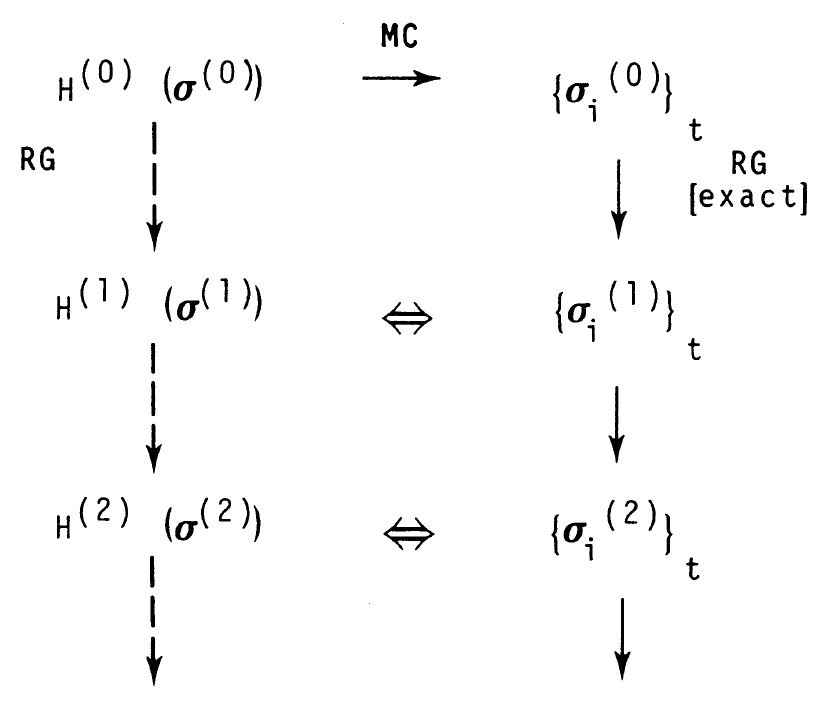
\includegraphics[width=0.5\textwidth]{idea}
\caption{Workflow of Swendsen's MCRG Approach}
\label{idea}
\end{figure}

After $n+1$ block spin transformations, an approximation to the matrix $T$ (denoted $T^{(n)}$) can be obtained via solving the set of linear equations
\begin{equation}
\sum_{\alpha}\frac{\partial \langle S_\gamma^{(n+1)}\rangle}{\partial K_\alpha^{(n+1)}}\cdot \frac{\partial K_\alpha^{(n+1)}}{\partial K_\beta^{(n)}} = \sum_{\alpha}\frac{\partial \langle S_\gamma^{(n+1)}\rangle}{\partial K_\alpha^{(n+1)}} T_{\alpha\beta} = \frac{\partial \langle S_\gamma^{(n+1)}\rangle}{\partial K_\beta^{(n)}} \label{LinRGMat}
\end{equation}
where everything except $T_{\alpha\beta}$ can be found via Monte Carlo simulations:
\begin{align}
\frac{\partial \langle S_\gamma^{(n+1)}\rangle}{\partial K_\alpha^{(n+1)}} &= \langle S_\gamma^{(n+1)}S_\alpha^{(n+1)}\rangle - \langle S_\gamma^{(n+1)} \rangle \langle S_\alpha^{(n+1)}\rangle\\
\frac{\partial \langle S_\gamma^{(n+1)}\rangle}{\partial K_\beta^{(n)}} &= \langle S_\gamma^{(n+1)}S_\beta^{(n)}\rangle - \langle S_\gamma^{(n+1)} \rangle \langle S_\beta^{(n)}\rangle
\end{align}

Then, the eigenvalues of $T^{(n)}$ are found and critical exponents evaluated.

The above approach introduce three sources of systematic error:
\renewcommand{\labelenumi}{(\roman{enumi})}
\begin{enumerate}
  \item \textbf{Finite system size}: We are using a \textit{truncated} renormalized Hamiltonian on the finite lattice as an approximation to what the \textit{full} renormalized Hamiltonian would have been on an infinite lattice. Only interactions that fit on the finite lattice are preserved by the RG transformations that we apply to spin configurations. For this approximation to be valid, the effective range of the \textit{full} renormalized Hamiltonian must be small compared with the size of the lattice. The validity of this approximation can be checked by performing the calculation on lattices of different sizes.
  \item \textbf{$T$ truncation}: $T$ is in principle infinite dimensional, but we can only keep track of a finite number, $N_c$, of coupling constants and calculate a small part of this matrix. The effects of adding additional coupling terms can be systematically checked.
  \item \textbf{$T^{(n)}$ not evaluated at the fixed point}: We calculate critical exponents based on the eigenvalues of $T^{(n)}$, but for any finite number of RG iterations $N_r$, $T^{(n)} \neq T$. The effect of evaluating the linearized transformation matrix off the fixed point can be checked by applying more RG transformations.
\end{enumerate}
In principle, we obtain exact results with the MCRG method in the thermodynamic limit and $N_c, N_r \rightarrow \infty$. However, Binder~\cite{Binder2014} claims that the convergence in practice is often much faster (which we shall see is indeed the case).

Additionally, our results will contain statistical error arising from using a finite number of Monte Carlo steps.



\section{Simulation Method}
Consider a system $\Omega$ of Ising spins $\sigma_i = \pm 1$ situated on a two dimensional $(d = 2)$ square lattice with linear dimension $L$ and lattice spacing 1. Then the total number of lattice sites is $N_s = L^2$. For simplicity, we start our analysis with a microscopic Hamiltonian with only nearest neighbor interactions:
\begin{equation}
\mathcal{H}^{(0)} = -\beta H_\Omega = K\sum_{\langle i,j\rangle} \sigma_i \sigma_j + h\sum_{i = 0}^{N_s} \sigma_i
\end{equation}
and set coupling constants to the known critical values $(K = K_c, h = 0)$. We use priodic boundary conditions. 

As discussed previously, because we have started on the critical manifold, as we repeatedly apply renormalization group transformations, the system will be moved towards the critical fixed point $\vec{K^*}$. After applying $n+1$ RG transformations, we numerically find the linearized RG matrix $T^{(n)}$ using Eq.~\ref{LinRGMat}-8, and find its eigenvalues in order to get estimates of critical exponents. As $n$ increases, we expect $T^{(n)}$ to approach its theoretical value $T$. (With finite precision numbers, we are not \textit{exactly} starting \textit{on} the critical manifold, but we still expect the system to move towards the fixed point $\vec{K^*}$ in the few RG iterations that we apply before diverging along one of the relevant directions.) 

For the standard Monte Carlo part, I choose to use Wolff's Algorithm~\cite{Wolff1989} to generate spin configurations, which performs well near the critical temperature $K_c$ and is less affected by critical slowing than the Metropolis-Hastings algorithm. Measurements of spin-spin correlation functions are taken every $\Delta_N$ steps to ensure that successive measurements are uncorrelated. The Monte Carlo simulation settings for four different lattice sizes are listed in Table~\ref{MCSettings}. A variety of lattice sizes are used because we want to examine how finite lattice sizes impact the renormalization group analysis. A number of independently seeded Monte Carlo simulations are run in order to obtain an estimate of the statistical uncertainty in our results.

\begin{table}[H]
\centering
\begin{tabular}{|c|c|c|c|c|} 
 \hline
 Lattice linear dimension $L$ & 64 & 32 & 16 & 8 \\ 
 \hline
 \# of independent MC runs: $N_R$ & 5&5&5&5\\
 Burn-in steps in each run:  $N_{warm}$ & $1\times 10^4$& $1\times 10^4$& $0.5\times 10^4$& $0.5\times 10^4$ \\ 
 Measurement steps each run: $N_{meas}$& $60\times 10^4$& $30\times 10^4$& $30\times 10^4$& $30\times 10^4$\\
 Cluster flips between measurements: $\Delta_N$ & 20 & 10 & 10 & 10 \\
 \hline
 Total \# of samples $N_{data} = N_R\times \frac{N_{meas}}{\Delta_{N}}$ & $15\times 10^4$& $15 \times 10^4$& $15\times 10^4$& $15\times 10^4$ \\
 \hline
 \end{tabular}
 \caption{\label{MCSettings}Monte Carlo simulation settings}
\end{table}

For the renormalization group analysis part, I use a simple block-spin transformation with scale factor $b = 2$. The renormalized block-spin value is determined by majority rule, with ties broken by random assignments of $+1$ and $-1$.  


Due to the $\{\sigma_i\} \leftrightarrow \{-\sigma_i\}$ symmetry of our model, we can analyze the even and odd coupling constants in the Hamiltonian separately. In other words, we can suppose that the block spin transformations do not mix even and odd coupling constant spaces. The largest (in magnitude) eigenvalue $\lambda_e$ of the linearized RG transformation matrix $T_{\alpha\beta}$ for even coupling constants produce the thermal exponent $y_T$ via:
\begin{equation}
y_T = \frac{\log \lambda_e}{\log b}
\end{equation}
The largest (in magnitude) eigenvalue $\lambda_o$ of the linearized RG transformation matrix $T_{\alpha\beta}$ for odd coupling constants  produce the megnetization exponent $y_H$ via:
\begin{equation}
y_H = \frac{\log \lambda_o}{\log b}
\end{equation}

From Onsager's exact solution \cite{Onsager1944} we know the exact critical exponents of the Ising model in two dimensions are $\nu = 1 ,\  \eta = 1/4$. So we expect to find~\cite{Goldenfeld1992}:
\begin{equation*}
y_T = 1/\nu = 1 \qquad y_H = d-\frac{d-2+\eta}{2}= \frac{15}{8}
\end{equation*}

In order to examine the effect of coupling constant space truncation in evaluating $T$ , coupling constants are added into the analysis one by one. [Equivalently, the $T^{(n)}$ matrices we obtain are of size $N_c$ by $N_c$, where $N_c$ is the number of coupling constants included in the RG analysis.] The even coupling constants that are one-by-one added to the RG analysis are given in Table~\ref{even}. 

\begin{table}[H]
\centering
\begin{tabular}{|c |c|} 
 \hline
\multicolumn{2}{|c|}{Even couplings} \\ 
 \hline
 Name & Meaning\\
 \hline
 $K_1$ & nearest neighbor $(0,0)$ - $(1,0)$\\
 $K_2$ & next-nearest neighbor $(0,0)$ - $(1,1)$\\
 $K_3$ & four spins on a plaquette $(1,0)$ - $(1,1)$ - $(0,1)$ - $(0,0)$\\
 $K_4$ & third nearest neighbor $(0,0)$ - $(2,0)$\\
 $K_5$ & fourth nearest neighbor $(0,0)$ - $(2,1)$\\
 $K_6$ & four spins on a sublattice plaquette $(2,0)$ - $(0,2)$ - $(-2,0)$ - $(0,-2)$\\
 $K_7$ & fifth nearest neighbor $(0,0)$ - $(2,2)$\\
 \hline
 \end{tabular}
 \caption{\label{even}First few even short range coupling constants that may be used in the RG analysis to find $y_T$}
\end{table}

The odd coupling constants that are one-by-one added to the RG analysis are given in Table~\ref{odd}. 

\begin{table}[H]
\centering
\begin{tabular}{|c |c|} 
 \hline
\multicolumn{2}{|c|}{Odd couplings} \\ 
 \hline
 Name & Meaning\\
 \hline
 $K_1$ & Magnetization $(0,0)$\\
 $K_2$ & Three spins on a plaquette $(0,0)$ - $(1,0)$ - $(1,1)$\\
 $K_3$ & Three spins in a row $(0,0)$ - $(1,0)$ - $(2,0)$\\
 $K_4$ & Three spins at an angle $(0,0)$ - $(1,0)$ - $(2,1)$\\
 \hline
 \end{tabular}
 \caption{\label{odd}First few odd short range coupling constants that may be used in the RG analysis to find $y_H$}
\end{table}



\section{Results}
All results for $y_T$ are shown in Table~\ref{yT} below. Estimated statistical uncertainties obtained from multiple independent MC runs are also given ($1\sigma$ confidence interval).
\begin{table}[H]
\centering
\begin{tabular}{|c|c|c|c|c|c|} 
\hline
 \multicolumn{2}{|c|}{ }& \multicolumn{4}{c|}{Lattice size L}\\
 \hline
 $n$ & $N_c$ & 64 & 32 & 16 & 8 \\
 \hline
 1 & 1 & 0.908(1) & 0.902(1)& 0.899(2) & 0.884(2)\\
 1 & 2 & 0.965(1) & 0.963(1) & 0.968(2)& 0.959(2)\\
 1 & 3 & 0.967(2) & 0.965(2)& 0.969(1) & 0.960(3)\\
 1 & 4 & 0.968(2) & 0.966(3) & 0.968(2) & 0.960(4)\\
 1 & 5 & 0.967(1) & 0.965(3) & 0.967(2) & 0.955(6)\\
 1 & 6 & 0.967(1) & 0.966(3) & 0.968(2) & 0.955(6)\\
 1 & 7 & 0.966(1) & 0.965(3) & 0.967(3) & 0.952(5)\\
 \hline
 2 & 1 & 0.965(3) & 0.953(2) & 0.934(3)&\\
 2 & 2 & 1.002(3) & 0.997(2) & 0.993(3)&\\
 2 & 3 & 1.004(3) & 0.998(2) & 0.995(4)&\\
 2 & 4 & 1.003(2) & 0.996(3) & 0.988(3)&\\
 2 & 5 & 1.002(2) & 0.996(3) & 0.981(5)&\\
 2 & 6 & 1.002(2) & 0.995(3) & 0.980(5)&\\
 2 & 7 & 1.001(2) & 0.996(3) & 0.976(5)&\\
 \hline
 3 & 1 & 0.955(1) & 0.944(1)& & \\
 3 & 2 & 0.997(1) & 0.998(1)& & \\
 3 & 3 & 0.999(1) & 0.999(2)& & \\
 3 & 4 & 0.999(1) & 0.998(2)& & \\
 3 & 5 & 0.997(2) & 0.994(3)& & \\
 3 & 6 & 0.997(2) & 0.993(4)& & \\
 3 & 7 & 0.997(2) & 0.993(2)& & \\
  \hline
 4 & 1 & 0.947(2) & & & \\
 4 & 2 & 1.000(2) & & & \\
 4 & 3 & 1.002(2) & & & \\
 4 & 4 & 0.993(4) & & & \\
 4 & 5 & 0.987(8) & & & \\
 4 & 6 & 0.986(8) & & & \\
 4 & 7 & 0.985(7) & & & \\
 \hline
 \end{tabular}
 \caption{\label{yT}thermal eigenvalue
exponent $y_T$ as a function of the number of RG iterations $N_r$, the number of coupling
constants in the RG analysis $N_c$}
\end{table}

All results for $y_H$ are shown in Table ~\ref{yH} below. Estimated statistical uncertainties obtained from multiple independent MC runs are also given ($1\sigma$ confidence interval).

\begin{table}[H]
\centering
\begin{tabular}{|c|c|c|c|c|c|} 
\hline
 \multicolumn{2}{|c|}{ }& \multicolumn{4}{c|}{Lattice size L}\\
 \hline
 $n$ & $N_c$ & 64 & 32 & 16 & 8 \\
 \hline
 1 & 1 & 1.88117(5) & 1.88070(7) & 1.8795(2) & 1.8766(6) \\
 1 & 2 & 1.88048(4) & 1.88031(7) & 1.8800(2) & 1.8793(6)\\
 1 & 3 & 1.88048(5) & 1.88028(7) & 1.8800(3) & 1.8793(6)\\
 1 & 4 & 1.88083(4) & 1.88064(8) & 1.8804(3) & 1.8798(6)\\
 \hline
 2 & 1 & 1.8758(1) & 1.8747(1) & 1.8720(2)& \\
 2 & 2 & 1.8760(1) & 1.8755(1) & 1.8749(3)& \\
 2 & 3 & 1.8760(1) & 1.8755(1) & 1.8749(2)& \\
 2 & 4 & 1.8760(1) & 1.8757(1) & 1.8749(2)& \\
 \hline
 3 & 1 & 1.8736(2) & 1.8705(4)& & \\
 3 & 2 & 1.8746(2) & 1.8734(5)& & \\
 3 & 3 & 1.8746(2) & 1.8732(4)& &\\
 3 & 4 & 1.8746(2) & 1.8733(4)& & \\
 \hline
 4 & 1 & 1.8709(3) & & & \\
 4 & 2 & 1.8737(3) & & & \\
 4 & 3 & 1.8737(3) & & &\\
 4 & 4 & 1.8738(3) & & & \\
 \hline
 \end{tabular}
 \caption{\label{yH}thermal eigenvalue
exponent $y_T$ as a function of the number of RG iterations $N_r$, the number of coupling
constants in the RG analysis $N_c$}
\end{table}

Both the $y_T$ and $y_H$ results listed above are consistent with Swendsen's result~\cite{SwendsenDetail} and close to exact values we expect. 

Looking at the $y_T$ results, we see that even with only 1 coupling constant considered, the MCRG method produces a good estimate of the critical exponent (error $< 10\%$). The inclusion of second nearest neighbor interactions, $K_2$, dramatically increases the accuracy of results, though the inclusion of more distant neighbors and four-spin couplings do not have a significant effect. As we expected, a larger lattice size $L$ gives more accurate results, though this effect is not as significant as increasing the number of coupling constants considered. As the number of RG iterations is increased, the results improve; except for when we consider 5-7 coupling constants. In these cases the results become slightly worse. This may be because as we increase the number of RG iterations, the renormalized lattice becomes smaller and finite size effects begin to distort the $T$ matrix when we include longer range coupling constants in our analysis.

All trends seen in Table~\ref{yT} are also present in the $y_H$ results. The $y_H$ results tend to have uniformly smaller deviations from the exact value, and lower statistical errors than $y_T$. Swendsen points out that ``this effect is characteristic of the magnetic eigenvalue, which is generally much less sensitive to size effects and the distance from the fixed point than the thermal eigenvalues."




\section{Conclusion}
A version of the Monte Carlo Renormalization Group method is successully implemented for the Ising Model on a two dimensional square lattice. Values for the critical exponents $y_H$ and $y_T$ are obtained. The influence of the size of lattice $L$, the number of $RG$ iterations $n$, and the number of coupling constants $N_c$ used in calculating $T^{(n)}$  on the results are discussed. The MCRG method works well for this particular simple model, although whether it is more broadly applicable to other systems remains to be seen. 

Some of the computing for this project was performed on the Sherlock cluster. I would like to thank Stanford University and the Stanford Research Computing Center for providing computational resources and support that contributed to these results.

\bibliographystyle{ieeetr}
\bibliography{paperref}


\end{document}
